\chapter{Device Characterization}

\section{Measurement Setup}

The device under test (DUT) consists of a planar RF structure enclosed in a metallic housing, containing three different configurations labeled A, B, and C. Each configuration was measured independently.

The DUT was characterized using a Vector Network Analyzer (VNA) in a one-port configuration, measuring the reflection coefficient $S_{11}$. This choice is dictated by the physical structure of the device, which is accessible from a single port.

\begin{figure}[H]
\centering
\includegraphics[width=0.7\linewidth]{Davides_Section/Dispabc/plots/dispabc.jpg}
\caption{Experimental setup showing the DUT connected to the VNA.}
\label{fig:dut_setup}
\end{figure}

A standard calibration procedure was applied prior to the measurements in order to remove the contribution of cables and connectors.

\section{Measured Response and Discussion}

The measured $|S_{11}|$ responses for the three configurations are reported in Figures below.

\begin{figure}[H]
\centering
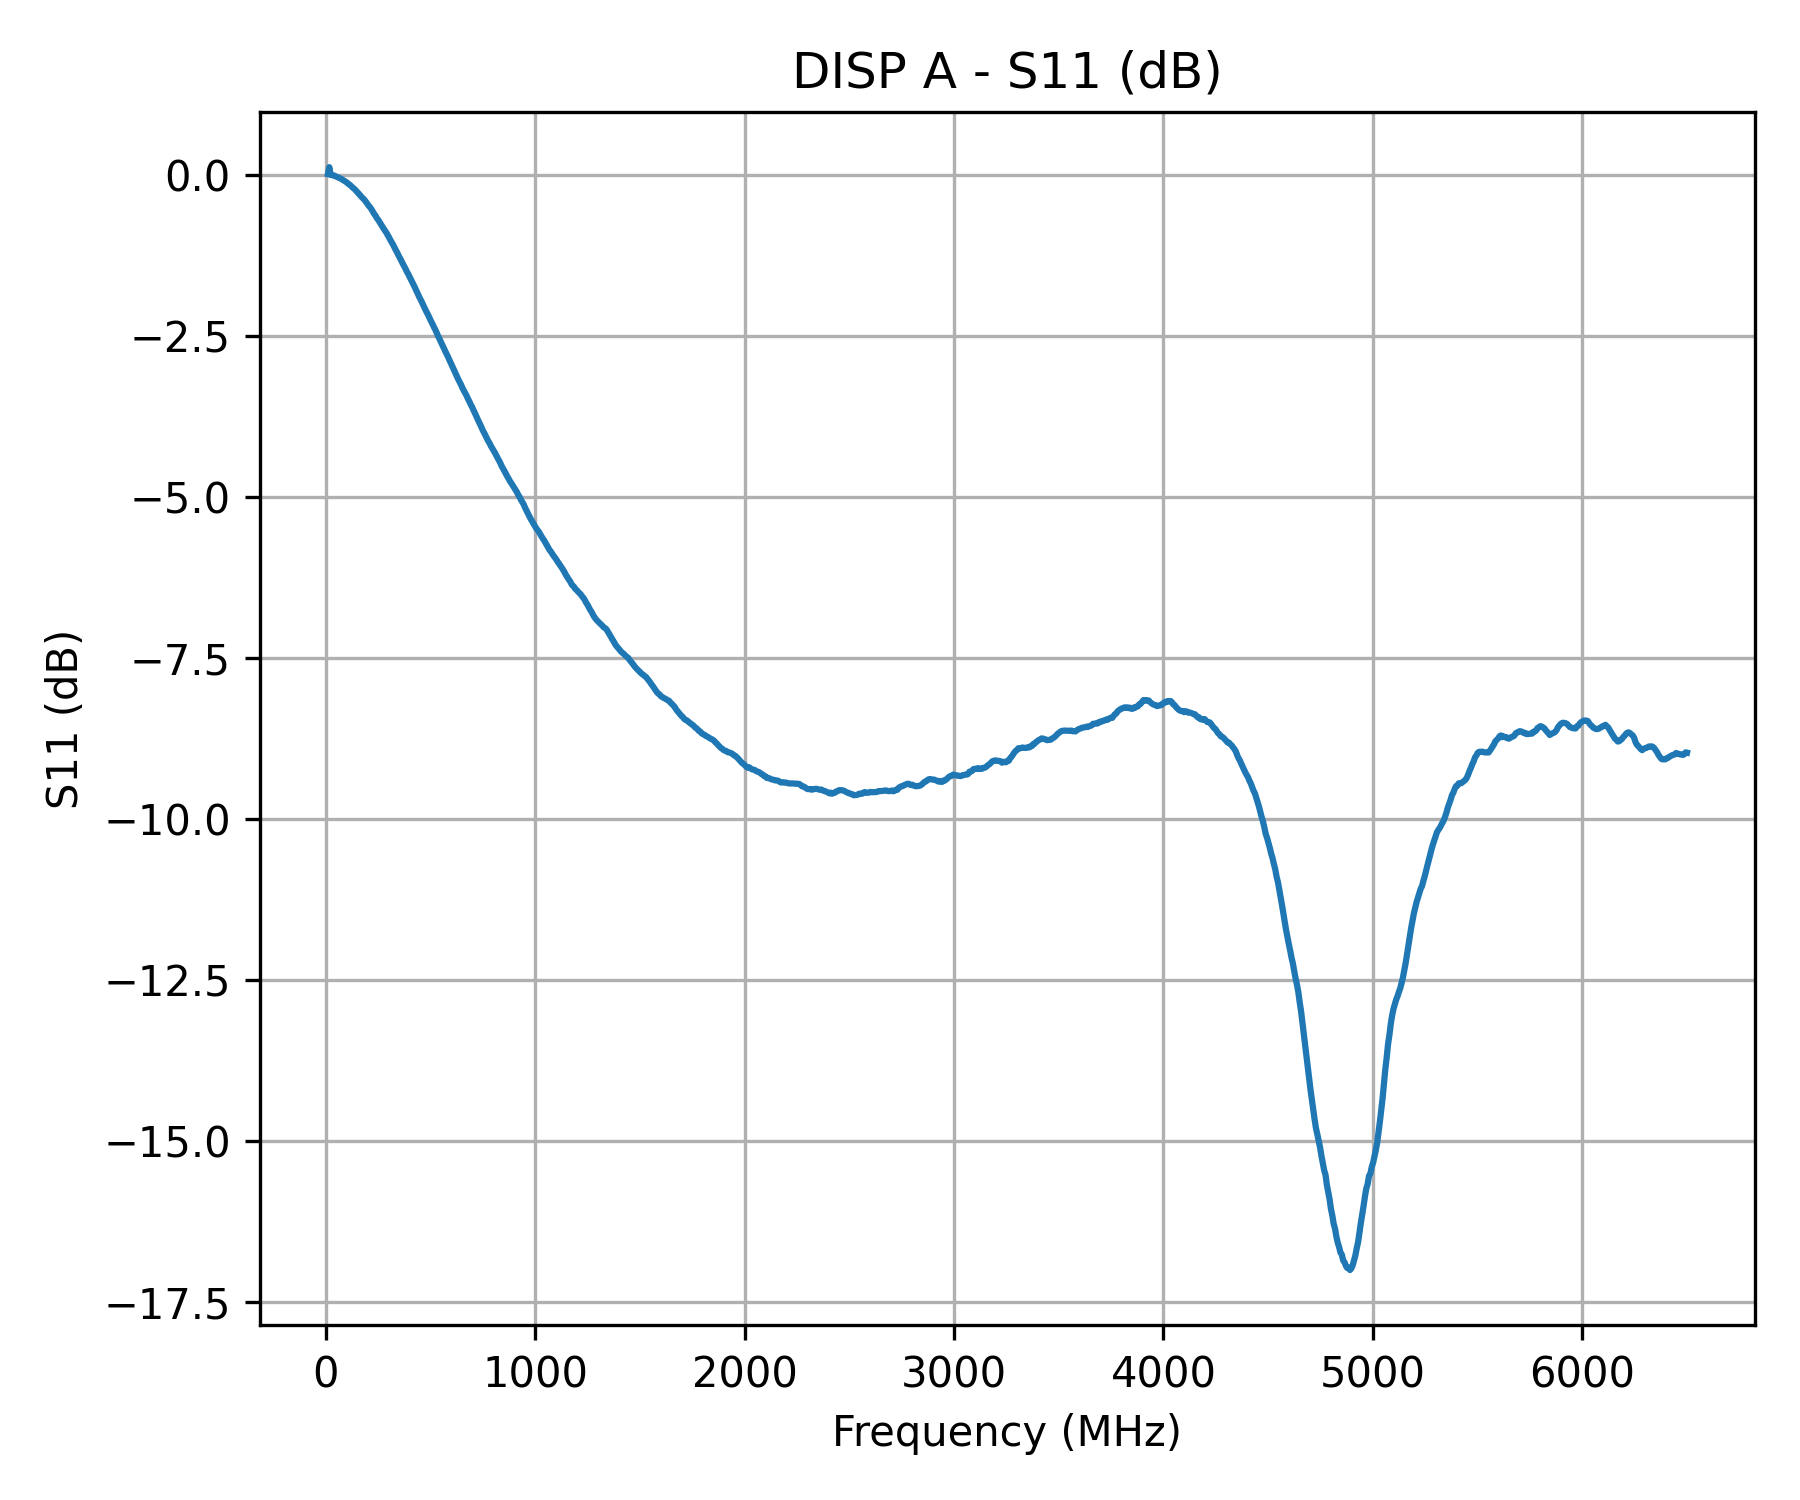
\includegraphics[width=0.8\linewidth]{Davides_Section/Dispabc/plots/disp_a.png}
\caption{$S_{11}$ magnitude for configuration A.}
\end{figure}

Configuration A exhibits a clear resonance around $5\,\mathrm{GHz}$, visible as a dip in the reflection coefficient reaching approximately $-17\,\mathrm{dB}$. The relatively broad shape of the dip indicates a moderate quality factor, suggesting non-negligible losses or weak confinement of the electromagnetic field.

\begin{figure}[H]
\centering
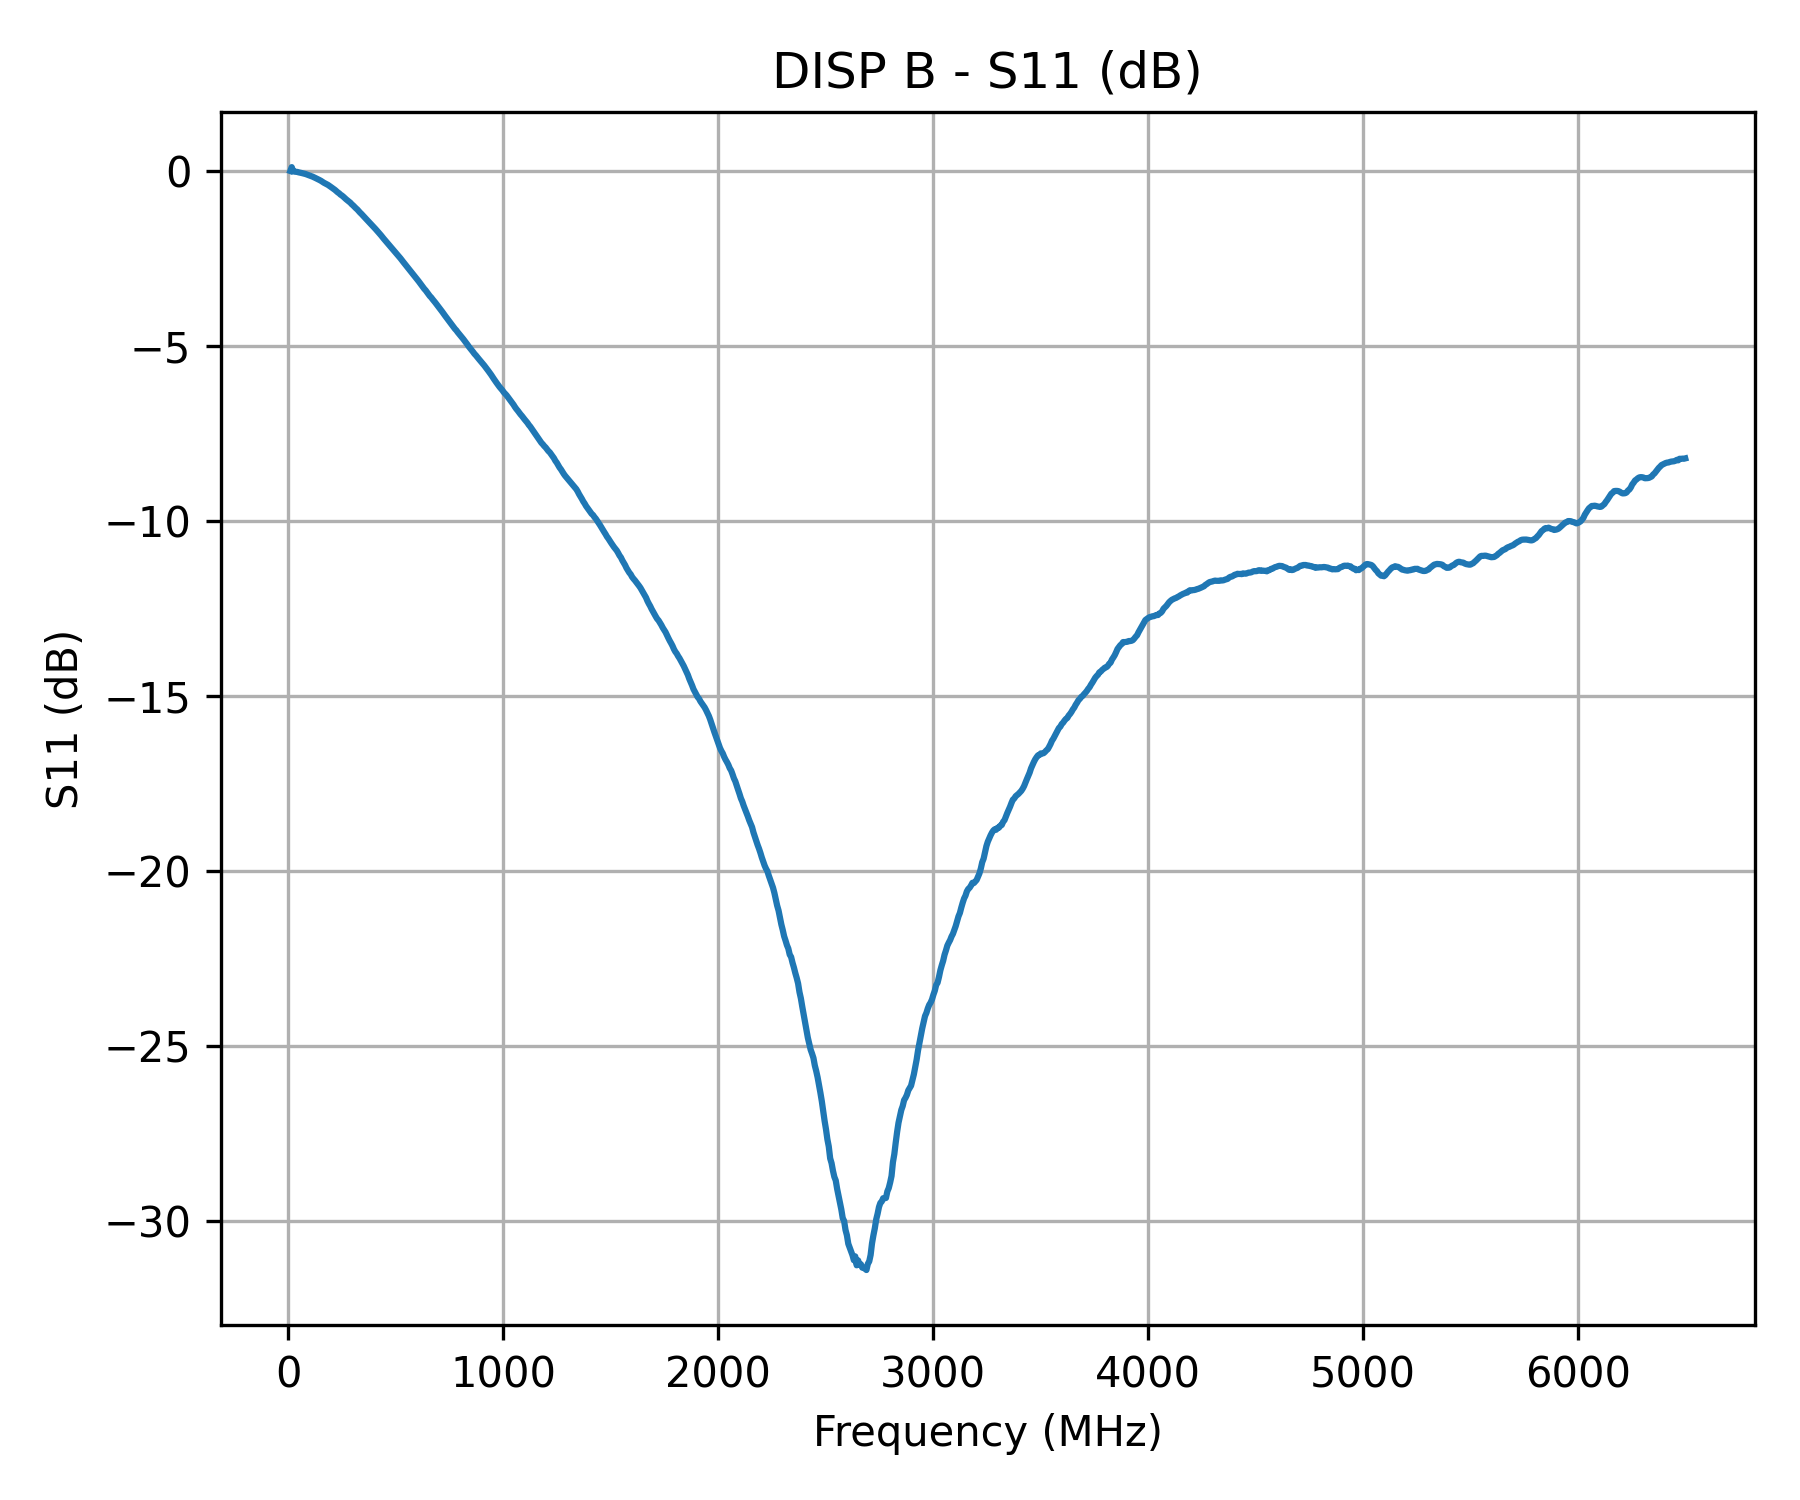
\includegraphics[width=0.8\linewidth]{Davides_Section/Dispabc/plots/disp_b.png}
\caption{$S_{11}$ magnitude for configuration B.}
\end{figure}

Configuration B shows a single, well-defined resonance around $2.7\,\mathrm{GHz}$, with a much deeper minimum (below $-30\,\mathrm{dB}$). This indicates a significantly better impedance matching at resonance and a higher quality factor, meaning that energy is more efficiently stored within the structure.

\begin{figure}[H]
\centering
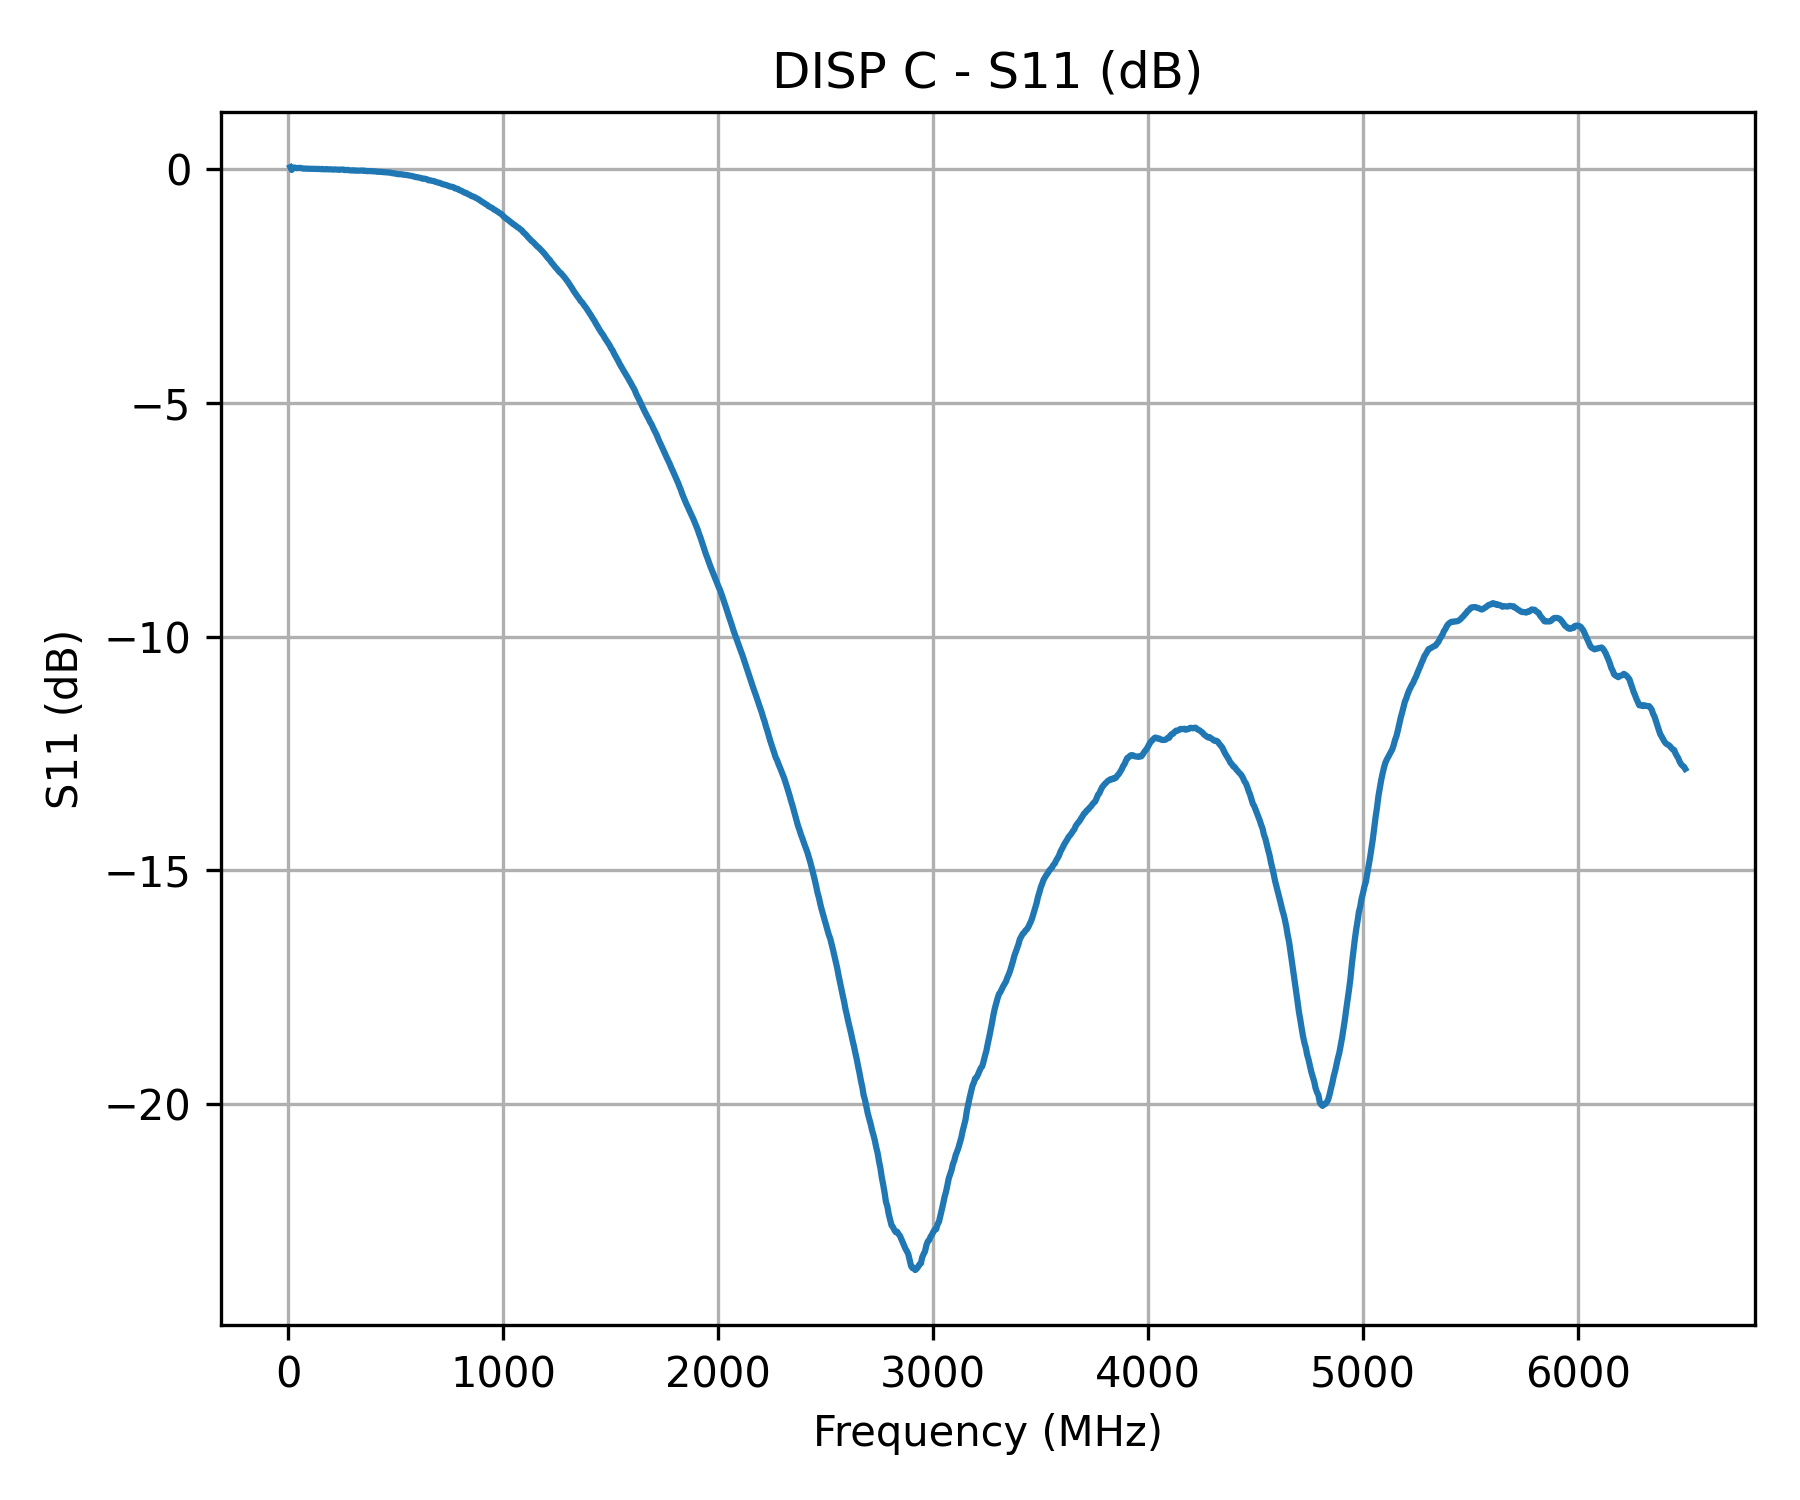
\includegraphics[width=0.8\linewidth]{Davides_Section/Dispabc/plots/disp_c.png}
\caption{$S_{11}$ magnitude for configuration C.}
\end{figure}

Configuration C exhibits a more complex behavior, with two distinct resonances around $3\,\mathrm{GHz}$ and $4.8\,\mathrm{GHz}$. This suggests the presence of multiple resonant modes, likely due to a more complex geometry or coupling between different sections of the structure.

\section{Physical Interpretation}

The observed responses are characteristic of reflective resonant structures implemented in planar technology, such as microstrip stub resonators.

In all configurations, the dips in $S_{11}$ correspond to frequencies at which the input impedance of the device approaches the characteristic impedance of the measurement system ($50\,\Omega$), resulting in reduced reflection. At these frequencies, the device stores electromagnetic energy, behaving as a resonator.

The variation in resonance frequency between configurations A, B, and C can be attributed to differences in the effective electrical length of the structures:
\begin{itemize}
    \item Configuration B resonates at the lowest frequency, indicating the largest effective length
    \item Configuration A resonates at higher frequency, corresponding to a shorter structure
    \item Configuration C supports multiple resonances, suggesting either higher-order modes or coupled resonators
\end{itemize}

Additionally, the depth and width of the resonant dips provide information about losses and coupling:
\begin{itemize}
    \item A deeper and sharper dip (configuration B) indicates stronger energy confinement and higher quality factor
    \item Broader resonances (configuration A) suggest increased losses or weaker confinement
\end{itemize}

\section{Conclusion}

The DUT behaves as a set of planar reflective resonators, with geometry-dependent resonance frequencies and quality factors. The one-port $S_{11}$ measurement is sufficient to identify the resonant behavior and distinguish between different configurations, including single-mode and multi-mode responses.